\section{Complex Time-Steps}
So far, we have restricted our time-steps to the real domain.\\
It has often proven useful to extend the analysis of a problem to the complex domain.\\
Motivated by a paper by \textit{George, Yung and Mangan}\cite{walking_into_the_complex_domain}, we will have a look at the stability of numerical methods when the chosen time-step is complex.\\
They state: \begin{quote} \textit {Most numerical methods for time integration use real time steps. Complex time steps provide an additional degree of freedom, as we can select the magnitude of the step in both the real and imaginary directions. By time stepping along specific paths in the complex plane, integrators can gain higher orders of accuracy or achieve expanded stability regions.}\end{quote}

\subsection{Complex 2-Step}
\begin{multicols}{2}
\par We want to take an overall step of size $h \in \bR$ comprised of two steps $z_1, z_2 \in \bC$ such that $z_1 + z_2 = h$.\\
We can set $z_1 = a + bi$ and $z_2 = h - a - bi$.\\

\par For analysing our numerical methods, we require a comparable implementation of the real step setup.\\
A real 2-step method where we take a step of size $\frac{h}{2}$ allows us to take two steps and go the same distance as the complex 2-step method.\\
We can write this real 2-step method as
\[y_{j+1} = s(\lambda, \frac{h}{2}) y_{j+\frac{1}{2}} = s(\lambda, \frac{h}{2}) s(\lambda, \frac{h}{2}) y_j = {s(\lambda, \frac{h}{2})}^{2} y_j\]

\par We can write the complex 2-step method as 
\[y_{j+1} = s(\lambda, z_1) y_{j+\frac{1}{2}} = s(\lambda, z_1) s(\lambda, z_2) y_j\]
\vspace*{\fill}
\columnbreak{}
% Triangle diagram
\begin{tikzpicture}
	\draw[->] (0,0) -- (8,0) node[right] {$Re$};
	\draw[->] (0,0) -- (0,8) node[above] {$Im$};
	\draw[-, color=orange] (0,0) -- (5,7) node[midway, shift={(-0.2,0)}, left] {$z_1$};
	\draw[-, color=orange] (5,7) -- (7,0) node[midway, shift={(0.1,0)}, right] {$z_1 + z_2$};
	\draw[color=purple] (0,0) -- (7,0) node[midway, below] {$h$};
\end{tikzpicture}
\end{multicols}


\subsection{Complex Conjugate Pairs}
\begin{multicols}{2}
% Triangle diagram
\begin{tikzpicture}
	\draw[->] (0,0) -- (7,0) node[right] {$Re$};
	\draw[->] (0,0) -- (0,4.5) node[above] {$Im$};
	\draw[-, color=orange] (0,0) -- (3,3.5) node[midway, shift={(-0.2,0)}, left] {$z$};
	\draw[-, color=orange] (3,3.5) -- (6,0) node[midway, shift={(0.1,0)}, right] {$z + \bar{z}$};
	\draw[-, color=purple] (0,0) -- (3,0) node[midway, below] {$\frac{h}{2}$};
	\draw[-, color=purple] (3,0) -- (6,0) node[midway, below] {$\frac{h}{2}$};
	\draw[-, color=blue] (3,0) -- (3,3.5) node[midway, right] {$b$};
\end{tikzpicture}
\columnbreak{}
\par When we restrict the exponential decay problem by $\lambda \in \bR$, we also find that $s(\lambda, z_1) s(\lambda, z_2) \in \bR$\\
This is because any value attained by $e^{\lambda t}$ is real.\\
This restricts the values of $z_1$ and $z_2$, as any imaginary terms in $s(\lambda, z_1) s(\lambda, z_2)$ must cancel out.\\

\par One particularly simple family of such complex pairs is defined by setting $a = \frac{h}{2}$\\
This necessitates $z_2 = \bar{z_1}$\\
We will refer to this family as the \term{complex conjugate step pairs}.\\
\end{multicols}

\subsection{Stability of 2-Step Methods for Complex Conjugate Step Pairs}
\par In this section we will compare the stability regions for the real and complex 2-step methods.\\
The real step size is given by $\frac{h}{2}$\\
The complex conjugate step pair is given by $z = \frac{h}{2} + bi$ and $\bar{z} = \frac{h}{2} - bi$\\
The plots in this section show the regions of stability $S = \{\lh : |s(\lambda, h)| \leq 1\}$ for the case where $b=a=\frac{\lh}{2}$\\
We will have a look at varying $b$ in a subsequent section.\\

\newpage
\subsubsection{Euler's Forward 2-Step}
\begin{theorem}\textbf{Euler's Forward Complex Step Pairs must be Conjugate for $\lambda \in \bR$}\\
\par For the exponential decay problem, $y=e^{\lambda t}$, let $\lambda \in \bR$\\
Let $z_1 = a_1 + b_1i$ and $z_2 = a_2 + b_2i$ be a complex step pair for Euler's Forward 2-Step Method.\\
Then we must have $z_2 = \bar{z_1}$\\
\par\textbf{Proof:}
\[\lambda \in \bR \implies y_{j}, y_{j+1} \in \bR\]
Euler's Forward 2-Step Method is given by:
\begin{flalign*}
	y_{j+1} &= s(\lambda, z_1) s(\lambda, z_2)\; y_j && \\
	&= \Big(1 + z_1\Big)\Big(1 + z_2\Big)\; y_j && \\
	&= \Big(1+a_1+b_1 i\Big)\Big(1+a_2+b_2 i\Big)\; y_j && \\
	&= \Bigg(\Big(1 + a_1 + a_2 +a_1 a_2 - b_1 b_2\Big) + \Big(b_1 + b_2 + a_1 b_2 + a_2 b_1\Big)i\Bigg)\; y_j &&
\end{flalign*}
\[y_{j+1} \in \bR \implies Im(y_{j+1}) = 0 \implies b_1 + b_2 + a_1 b_2 + a_2 b_1 = 0 \implies (1+a_1)b_2 + (1+a_2)b_1 = 0\]
\[z_1+z_2 = h \in \bR \implies a_1+a_2 + (b_1+b_2)i = h \implies b_1+b_2 = 0 \implies b_1 = -b_2\]
\[(1+a_1)b_2 + (1+a_2)b_1 = 0 \implies (1+a_1)b_2 - (1+a_2)b_2 = 0 \implies b_2 = 0 = b_1 \text{ or } a_1 = a_2\]
Thus, $z_1, z_2 \in \bC \implies a_1 = a_2$ and $b_1 = -b_2$
\[\therefore z_1 = a_1 + b_1i \text{ and } z_2 = a_1 - b_1i \implies z_2 = \bar{z_1} \qquad\square\]
\end{theorem}
\begin{multicols}{2}
\begin{center}
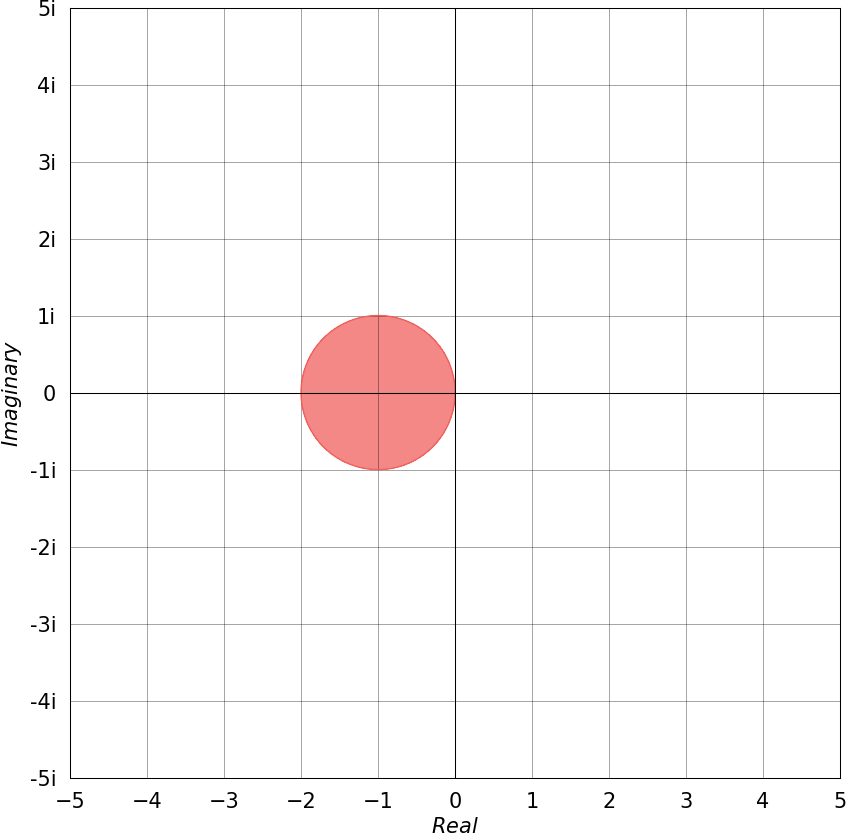
\includegraphics[width=0.49\textwidth]{Stability Regions/Graphs/Real VS Complex Comparison/Euler's Forward.png}
Appendix~\ref{appendix:real_vs_complex_stability} contains the code for this graph.
\end{center}
\columnbreak{}

\textbf{Euler's Forward 2-Step $\bR$}
\begin{flalign*}
	y_{j+1} &= {\Big(1+ \frac{\lh}{2}\Big)}^2 y_j && \\
	\implies &s_{_{\bR}}(\lambda, h) = 1 + \lh + \frac{{(\lh)}^2}{4} &&
\end{flalign*}

\textbf{Euler's Forward 2-Step $\bC$}
\begin{flalign*}
	y_{j+1} &= \Big(1 + z\Big)\Big(1 + \bar{z}\Big) y_j && \\
	    &= \Big(1 + \frac{\lambda h}{2} + bi\Big)\Big(1 + \frac{\lambda h}{2} - bi\Big) y_j && \\
	    &= \bigg(\Big{(1 + \frac{\lambda h}{2}\Big)}^2 + b^2\bigg) y_j && \\
    \implies &s_{_{\mathbb{C}}}(\lambda, h) = 1 + \lambda h + \frac{{(\lambda h)}^2}{4} + b^2 && \\
    \implies &s_{_{\mathbb{C}}}(\lambda, h) = s_{_{\mathbb{R}}}(\lambda, h) + b^2 &&
\end{flalign*}

\vspace*{\fill}
\end{multicols}

\par As $b \in \bR$, $s_{_{\mathbb{C}}}(\lambda, h) \geq s_{_{\mathbb{R}}}(\lambda, h)$\\
This means the stability region for the complex 2-step method is smaller than that of the real 2-step method; there are less values of $\lh$ for which the complex 2-step method is stable.\\
$S_{_{\mathbb{C}}}$ is smaller than $S_{_{\mathbb{R}}}$\\
The diagram above illustrates the case where $b = a = \frac{\lh}{2}$\\
In this case, we have 
\[s_{_{\mathbb{R}}}(\lambda, h) = 1 + \lh + \frac{{(\lambda h)}^2}{4} = M(y) + \mathcal{O}({(\lh)}^2)\]
while
\[s_{_{\mathbb{C}}}(\lambda, h) = 1 + \lh + \frac{{(\lambda h)}^2}{2} = M(y) + \mathcal{O}({(\lh)}^3)\]
The complex 2-step method has a higher order of accuracy than the real 2-step method, with the trade-off of a smaller stability region.\\

\par We can do the same kind of analysis for other Numerical Methods.\\
The same derivations and diagrams for the Backward Euler and Runge-Kutta 4 methods follow.\\

\subsubsection{Euler's Backward 2-Step}
\begin{theorem}\textbf{Euler's Backward Complex Step Pairs must be Conjugate for $\lambda \in \bR$}\\
\par For the exponential decay problem, $y=e^{\lambda t}$, let $\lambda \in \bR$\\
Let $z_1 = a_1 + b_1i$ and $z_2 = a_2 + b_2i$ be a complex step pair for Euler's Backward 2-Step Method.\\
Then we must have $z_2 = \bar{z_1}$\\
\par\textbf{Proof:}
\[\lambda \in \bR \implies y_{j}, y_{j+1} \in \bR\]
Euler's Backward 2-Step Method is given by:
\begin{flalign*}
	y_{j+1} &= s(\lambda, z_1) s(\lambda, z_2)\; y_j && \\
	&= \Big(\frac{1}{1-z_1}\Big)\Big(\frac{1}{1-z_2}\Big)\; y_j && \\
        &= \Big(\frac{1}{(1-z_1)(1-z_2)}\Big)\; y_j &&
\end{flalign*}
\begin{flalign*}
	(1-z_1)(1-z_2) &= (1-a_1-b_1i)(1-a_2-b_2i) &&\\
		       &= \big[1-a_1-a_2+a_1 a_2-b_1 b_2\big] + \big[a_1 b_2 + a_2 b_1 - b_1 - b_2\big]i && \\
		       &= \big[(a_1-1)(a_2-1)-b_1 b_2\big] + \big[b_1(a_2-1) + b_2(a_1-1)\big]i && 
\end{flalign*}
\[y_{j+1} \in \bR \implies Im(y_{j+1}) = 0 \implies b_1(a_2-1) + b_2(a_1-1) = 0\]
\[z_1+z_2 = h \in \bR \implies a_1+a_2 + (b_1+b_2)i = h \implies b_1+b_2 = 0 \implies b_1 = -b_2\]
\[b_1(a_2-1) + b_2(a_1-1) = 0 \implies b_1(a_2-1) - b_1(a_1-1) = 0 \implies b_1 = 0 = b_2 \text{ or } a_1 = a_2\]
Thus, $z_1, z_2 \in \bC \implies a_1 = a_2$ and $b_1 = -b_2$
\[\therefore z_1 = a_1 + b_1i \text{ and } z_2 = a_1 - b_1i \implies z_2 = \bar{z_1} \qquad\square\]
\end{theorem}
\begin{multicols}{2}
\begin{center}
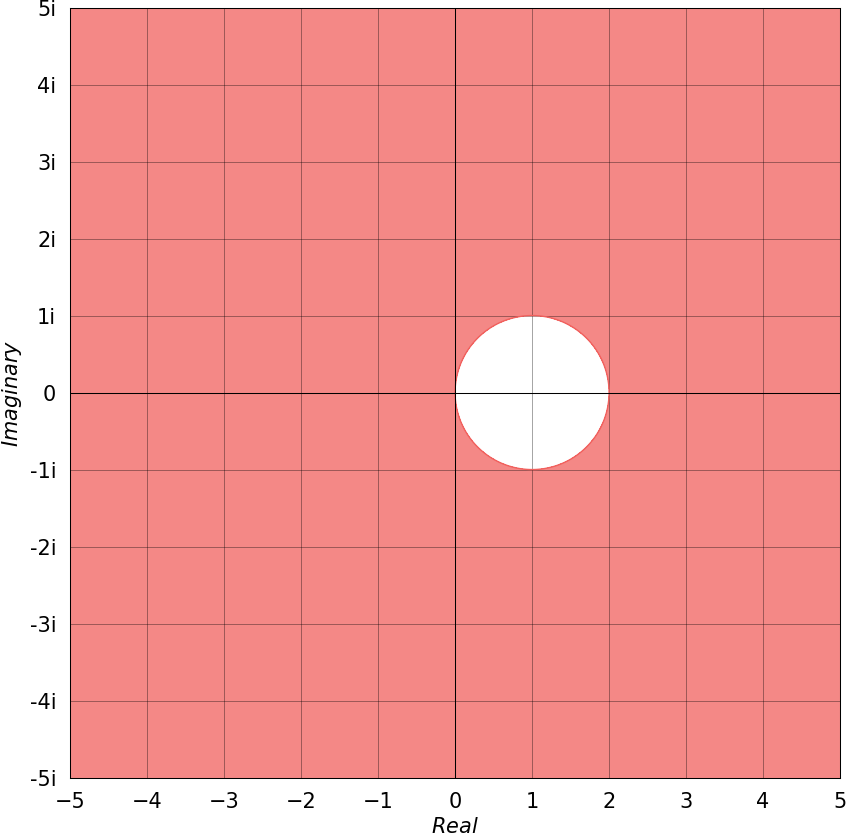
\includegraphics[width=0.49\textwidth]{Stability Regions/Graphs/Real VS Complex Comparison/Euler's Backward.png}
Appendix~\ref{appendix:real_vs_complex_stability} contains the code for this graph.
\end{center}
\columnbreak{}

\textbf{Euler's Backward 2-Step $\bR$}
\begin{flalign*}
	y_{j+1} &= {\bigg(\frac{1}{1-\frac{\lh}{2}}\bigg)}^2 y_j && \\
	\implies & s_{\bR}(\lambda, h) = \frac{1}{1 - \lh + \frac{{(\lh)}^2}{4}} &&
\end{flalign*}

\textbf{Euler's Backward 2-Step $\bC$}
\begin{flalign*}
	y_{j+1} &= \bigg(\frac{1}{1-\frac{\lh}{2}+bi}\bigg)\bigg(\frac{1}{1-\frac{\lh}{2}-bi}\bigg)y_j && \\
    \implies &s_{\bC}(\lambda, h) = \frac{1}{1 - \lh + \frac{{(\lh)}^2}{4} + b^2} && \\
\end{flalign*}
\par Again, $b \in \bR$, so this time,\\
$s_{_{\mathbb{C}}}(\lambda, h) \leq s_{_{\mathbb{R}}}(\lambda, h) \implies S_{_{\mathbb{C}}}$ is larger than $S_{_{\mathbb{R}}}$\\
\vspace*{\fill}
\end{multicols}

\newpage
\subsubsection{Runge-Kutta 4 2-Step}
\begin{conjecture}\textbf{Runge-Kutta 4 Complex Step Pairs must be Conjugate for $\lambda \in \bR$}\\
	\par This is left as a conjecture for now, as the expansion we did in the other two proofs is much more complicated for the Runge-Kutta 4 method.\\
	The proof is left as an exercise in futility for the reader.\\
	Have a look at Appendix~\ref{appendix:rk4_conjecture} for the full expansion of the stability function for the Runge-Kutta 4 method,\\
	if long algebraic expressions are your flavour of masochism.\\
\end{conjecture}
\begin{multicols}{2}
\begin{center}
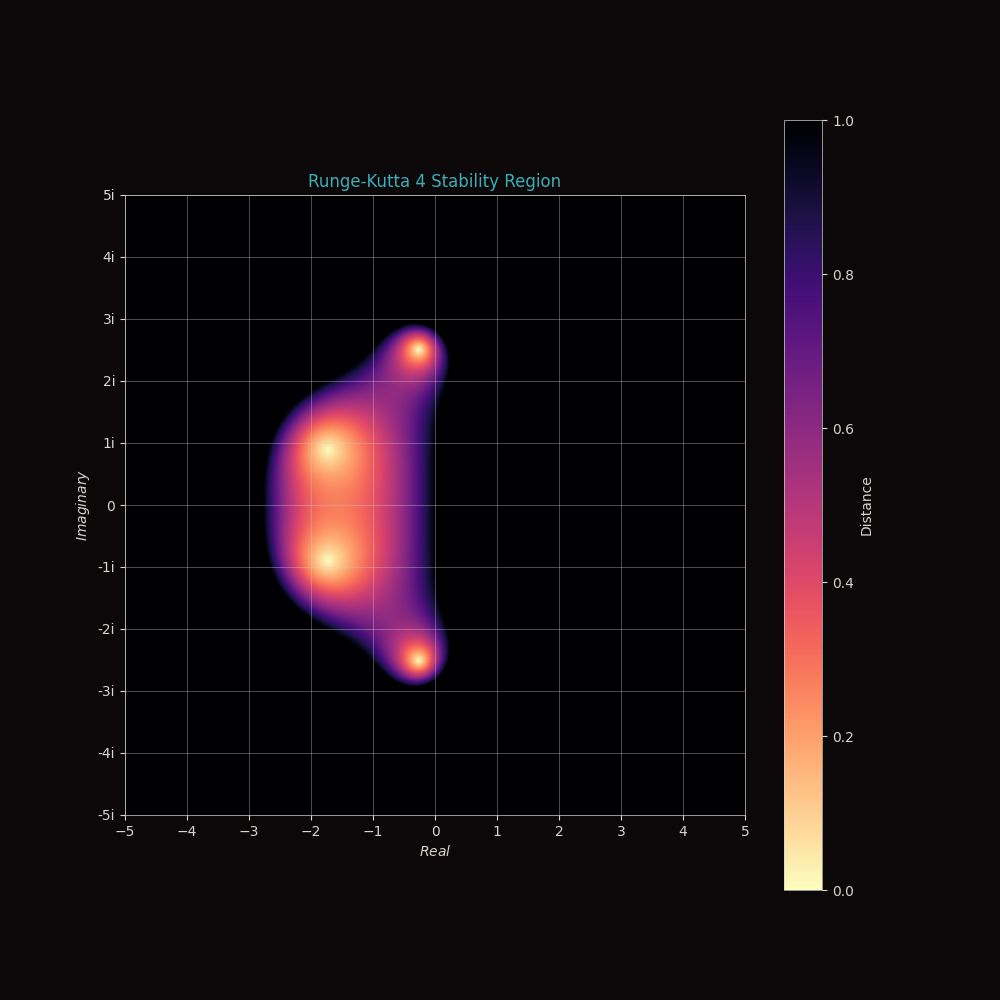
\includegraphics[width=0.49\textwidth]{Stability Regions/Graphs/Real VS Complex Comparison/Runge-Kutta 4.png}
Appendix~\ref{appendix:real_vs_complex_stability} contains the code for this graph.
\end{center}
\columnbreak{}

\textbf{Runge-Kutta 4 2-Step $\bR$}
\begin{flalign*} 
	y_{j+1} &= {\bigg(1+\frac{\lh}{2}+\frac{{(\frac{\lh}{2})}^2}{2}+\frac{{(\frac{\lh}{2})}^3}{6}+\frac{{(\frac{\lh}{2})}^4}{24}\bigg)}^2 y_j && \\
	y_{j+1} &= \bigg(1+\lh+\frac{{(\lh)}^2}{2}+\frac{{(\lh)}^3}{6}+\frac{{(\lh)}^4}{24} && \\
            &\quad\,\,\,\,+\frac{{(\lh)}^5}{128}+\frac{5{(\lh)}^6}{4608}+\frac{{(\lh)}^7}{9216}+\frac{{(\lh)}^8}{147456}\bigg) y_j && \\
	\implies &s_{_{\bR}}(\lambda, h) = 1+\lh+\frac{{(\lh)}^2}{2}+\frac{{(\lh)}^3}{6}+\frac{{(\lh)}^4}{24} && \\
            &\qquad\qquad\quad+\frac{{(\lh)}^5}{128}+\frac{5{(\lh)}^6}{4608}+\frac{{(\lh)}^7}{9216}+\frac{{(\lh)}^8}{147456} &&
\end{flalign*}

\textbf{Runge-Kutta 4 2-Step $\bC$}
\[y_{j+1} = \bigg(1+z+\frac{z^2}{2}+\frac{z^3}{6}+\frac{z^4}{24}\bigg)\bigg(1+\bar{z}+\frac{\bar{z}^2}{2}+\frac{\bar{z}^3}{6}+\frac{\bar{z}^4}{24}\bigg) y_j\]

\end{multicols}
$\implies s_{_{\bC}}(\lambda, h) = 1 + \lh + \frac{\lh^2}{2} + \frac{\lh^3}{6} + \frac{\lh^4}{24} + \frac{\lh^5}{128} + \frac{5 \lh^6}{4608} + \frac{\lh^7}{9216} + \frac{\lh^8}{147456} + \frac{b^2 \lh^3}{48} + \frac{b^2 \lh^4}{128} + \frac{b^2 \lh^5}{768} + \frac{b^2 \lh^6}{9216} + \frac{b^4 \lh}{24} - \frac{b^4 \lh^2}{96} + \frac{b^4 \lh^3}{192} + \frac{b^4 \lh^4}{1536} - \frac{b^6}{72} + \frac{b^6 \lh}{144} + \frac{b^6 \lh^2}{576} + \frac{b^8}{576}$
\newpage
\subsection{Varying b for Complex Conjugate Step Pairs}
\par As mentioned earlier, we need not only focus on the case where $b = \frac{\lh}{2}$\\
We can vary $b$ and see how the stability regions change.\\
In the cases below, we have preserved $a = \frac{\lh}{2}$\\
Consequently, these are still complex conjugate step pairs.\\
Videos showing the stability regions for varying $b$ values can be found in the \textit{GitHub Repository}\cite{GitHub_Repo} for this project.\\
These videos were created frame-by-frame using the script in Appendix~\ref{appendix:video_frames}.\\
The frames were stiched together using the script in Appendix~\ref{appendix:frames_to_video}.\\
Below are some of the video frames for each method.\\
\textbf{Observations:}
\begin{itemize}
	\item[$\cdot$] The stability region for complex conjugate pairs is always symmetric accross the real axis.
	      
	\item[$\cdot$] As $b$ increases, the stability region shrinks for explicit methods and grows for implicit methods.\\
        This can be seen quite simply in the $s_{_{\bC}}(\lambda, h)$ equations for Euler's Forward and Backward methods.

        \item[$\cdot$] The stability region for Euler's Backward Method is the complement of that for Euler's Forward Method, after it has been reflected across the imaginary axis.

\end{itemize}
\subsubsection{Euler's Forward}
\vspace*{-0.65cm}
\begin{multicols}{3}
	\begin{center}
		\includegraphics[width=0.32\textwidth]{Stability Regions/Videos/Varied b/Euler's Forward/a=0.5/frames/0200.png}
	\end{center}
	\columnbreak{}
	\begin{center}
		\includegraphics[width=0.32\textwidth]{Stability Regions/Videos/Varied b/Euler's Forward/a=0.5/frames/0350.png}
	\end{center}
	\columnbreak{}
	\begin{center}
		\includegraphics[width=0.32\textwidth]{Stability Regions/Videos/Varied b/Euler's Forward/a=0.5/frames/0500.png}
	\end{center}
\end{multicols}
\subsubsection{Euler's Backward}
\vspace*{-0.65cm}
\begin{multicols}{3}
	\begin{center}
		\includegraphics[width=0.32\textwidth]{Stability Regions/Videos/Varied b/Euler's Backward/a=0.5/frames/0200.png}
	\end{center}
	\columnbreak{}
	\begin{center}
		\includegraphics[width=0.32\textwidth]{Stability Regions/Videos/Varied b/Euler's Backward/a=0.5/frames/0350.png}
	\end{center}
	\columnbreak{}
	\begin{center}
		\includegraphics[width=0.32\textwidth]{Stability Regions/Videos/Varied b/Euler's Backward/a=0.5/frames/0500.png}
	\end{center}
\end{multicols}
\subsubsection{Runga-Kutta 4}
\vspace*{-0.65cm}
\begin{multicols}{3}
	\begin{center}
		\includegraphics[width=0.32\textwidth]{Stability Regions/Videos/Varied b/Runge-Kutta 4/a=0.5/frames/0200.png}
	\end{center}
	\columnbreak{}
	\begin{center}
		\includegraphics[width=0.32\textwidth]{Stability Regions/Videos/Varied b/Runge-Kutta 4/a=0.5/frames/0350.png}
	\end{center}
	\columnbreak{}
	\begin{center}
		\includegraphics[width=0.32\textwidth]{Stability Regions/Videos/Varied b/Runge-Kutta 4/a=0.5/frames/0500.png}
	\end{center}
\end{multicols}
\newpage
\subsection{Varying a}
\par We can also vary $a$ and see how the stability regions change.\\
This falls outside the scope of complex conjugate step pairs.\\
Consequently, these stability regions can only be interpreted for $\lambda \in \bC\setminus\bR$ (If you believe Conjecture 1).\\
In the cases below, we have set $b = \frac{\lh}{2}$\\
Videos showing the stability regions for varying $a$ values can be found in the \textit{GitHub Repository}\cite{GitHub_Repo} for this project.\\
The same process was followed as in the previous section:\\
The videos were created frame-by-frame using the script in Appendix~\ref{appendix:video_frames}.\\
The frames were stiched together using the script in Appendix~\ref{appendix:frames_to_video}.\\
Below are some of the video frames for each method.\\
\textbf{Observations:}
\begin{itemize}
	\item[$\cdot$] The stability region for varying $a$ values is not symmetric across the real axis, except for the case where $a = 0.5$.
	\item[$\cdot$] The stability regions for $a = 0.5 \pm \alpha$ are symmetric to each other across the real axis for any $|\alpha| < 0.5$.
	\item[$\cdot$] The stability region for Euler's Backward Method is the complement of that for Euler's Forward Method, after it has been reflected across the imaginary axis.
\end{itemize}
\subsubsection{Euler's Forward}
\vspace*{-0.65cm}
\begin{multicols}{3}
	\begin{center}
		\includegraphics[width=0.32\textwidth]{Stability Regions/Videos/Varied a/Euler's Forward/b=0.5/frames/0200.png}
	\end{center}
	\columnbreak{}
	\begin{center}
		\includegraphics[width=0.32\textwidth]{Stability Regions/Videos/Varied a/Euler's Forward/b=0.5/frames/0500.png}
	\end{center}
	\columnbreak{}
	\begin{center}
		\includegraphics[width=0.32\textwidth]{Stability Regions/Videos/Varied a/Euler's Forward/b=0.5/frames/0800.png}
	\end{center}
\end{multicols}
\subsubsection{Euler's Backward}
\vspace*{-0.65cm}
\begin{multicols}{3}
	\begin{center}
		\includegraphics[width=0.32\textwidth]{Stability Regions/Videos/Varied a/Euler's Backward/b=0.5/frames/0200.png}
	\end{center}
	\columnbreak{}
	\begin{center}
		\includegraphics[width=0.32\textwidth]{Stability Regions/Videos/Varied a/Euler's Backward/b=0.5/frames/0500.png}
	\end{center}
	\columnbreak{}
	\begin{center}
		\includegraphics[width=0.32\textwidth]{Stability Regions/Videos/Varied a/Euler's Backward/b=0.5/frames/0800.png}
	\end{center}
\end{multicols}
\subsubsection{Runga-Kutta 4}
\vspace*{-0.65cm}
\begin{multicols}{3}
	\begin{center}
		\includegraphics[width=0.32\textwidth]{Stability Regions/Videos/Varied a/Runge-Kutta 4/b=0.5/frames/0350.png}
	\end{center}
	\columnbreak{}
	\begin{center}
		\includegraphics[width=0.32\textwidth]{Stability Regions/Videos/Varied a/Runge-Kutta 4/b=0.5/frames/0500.png}
	\end{center}
	\columnbreak{}
	\begin{center}
		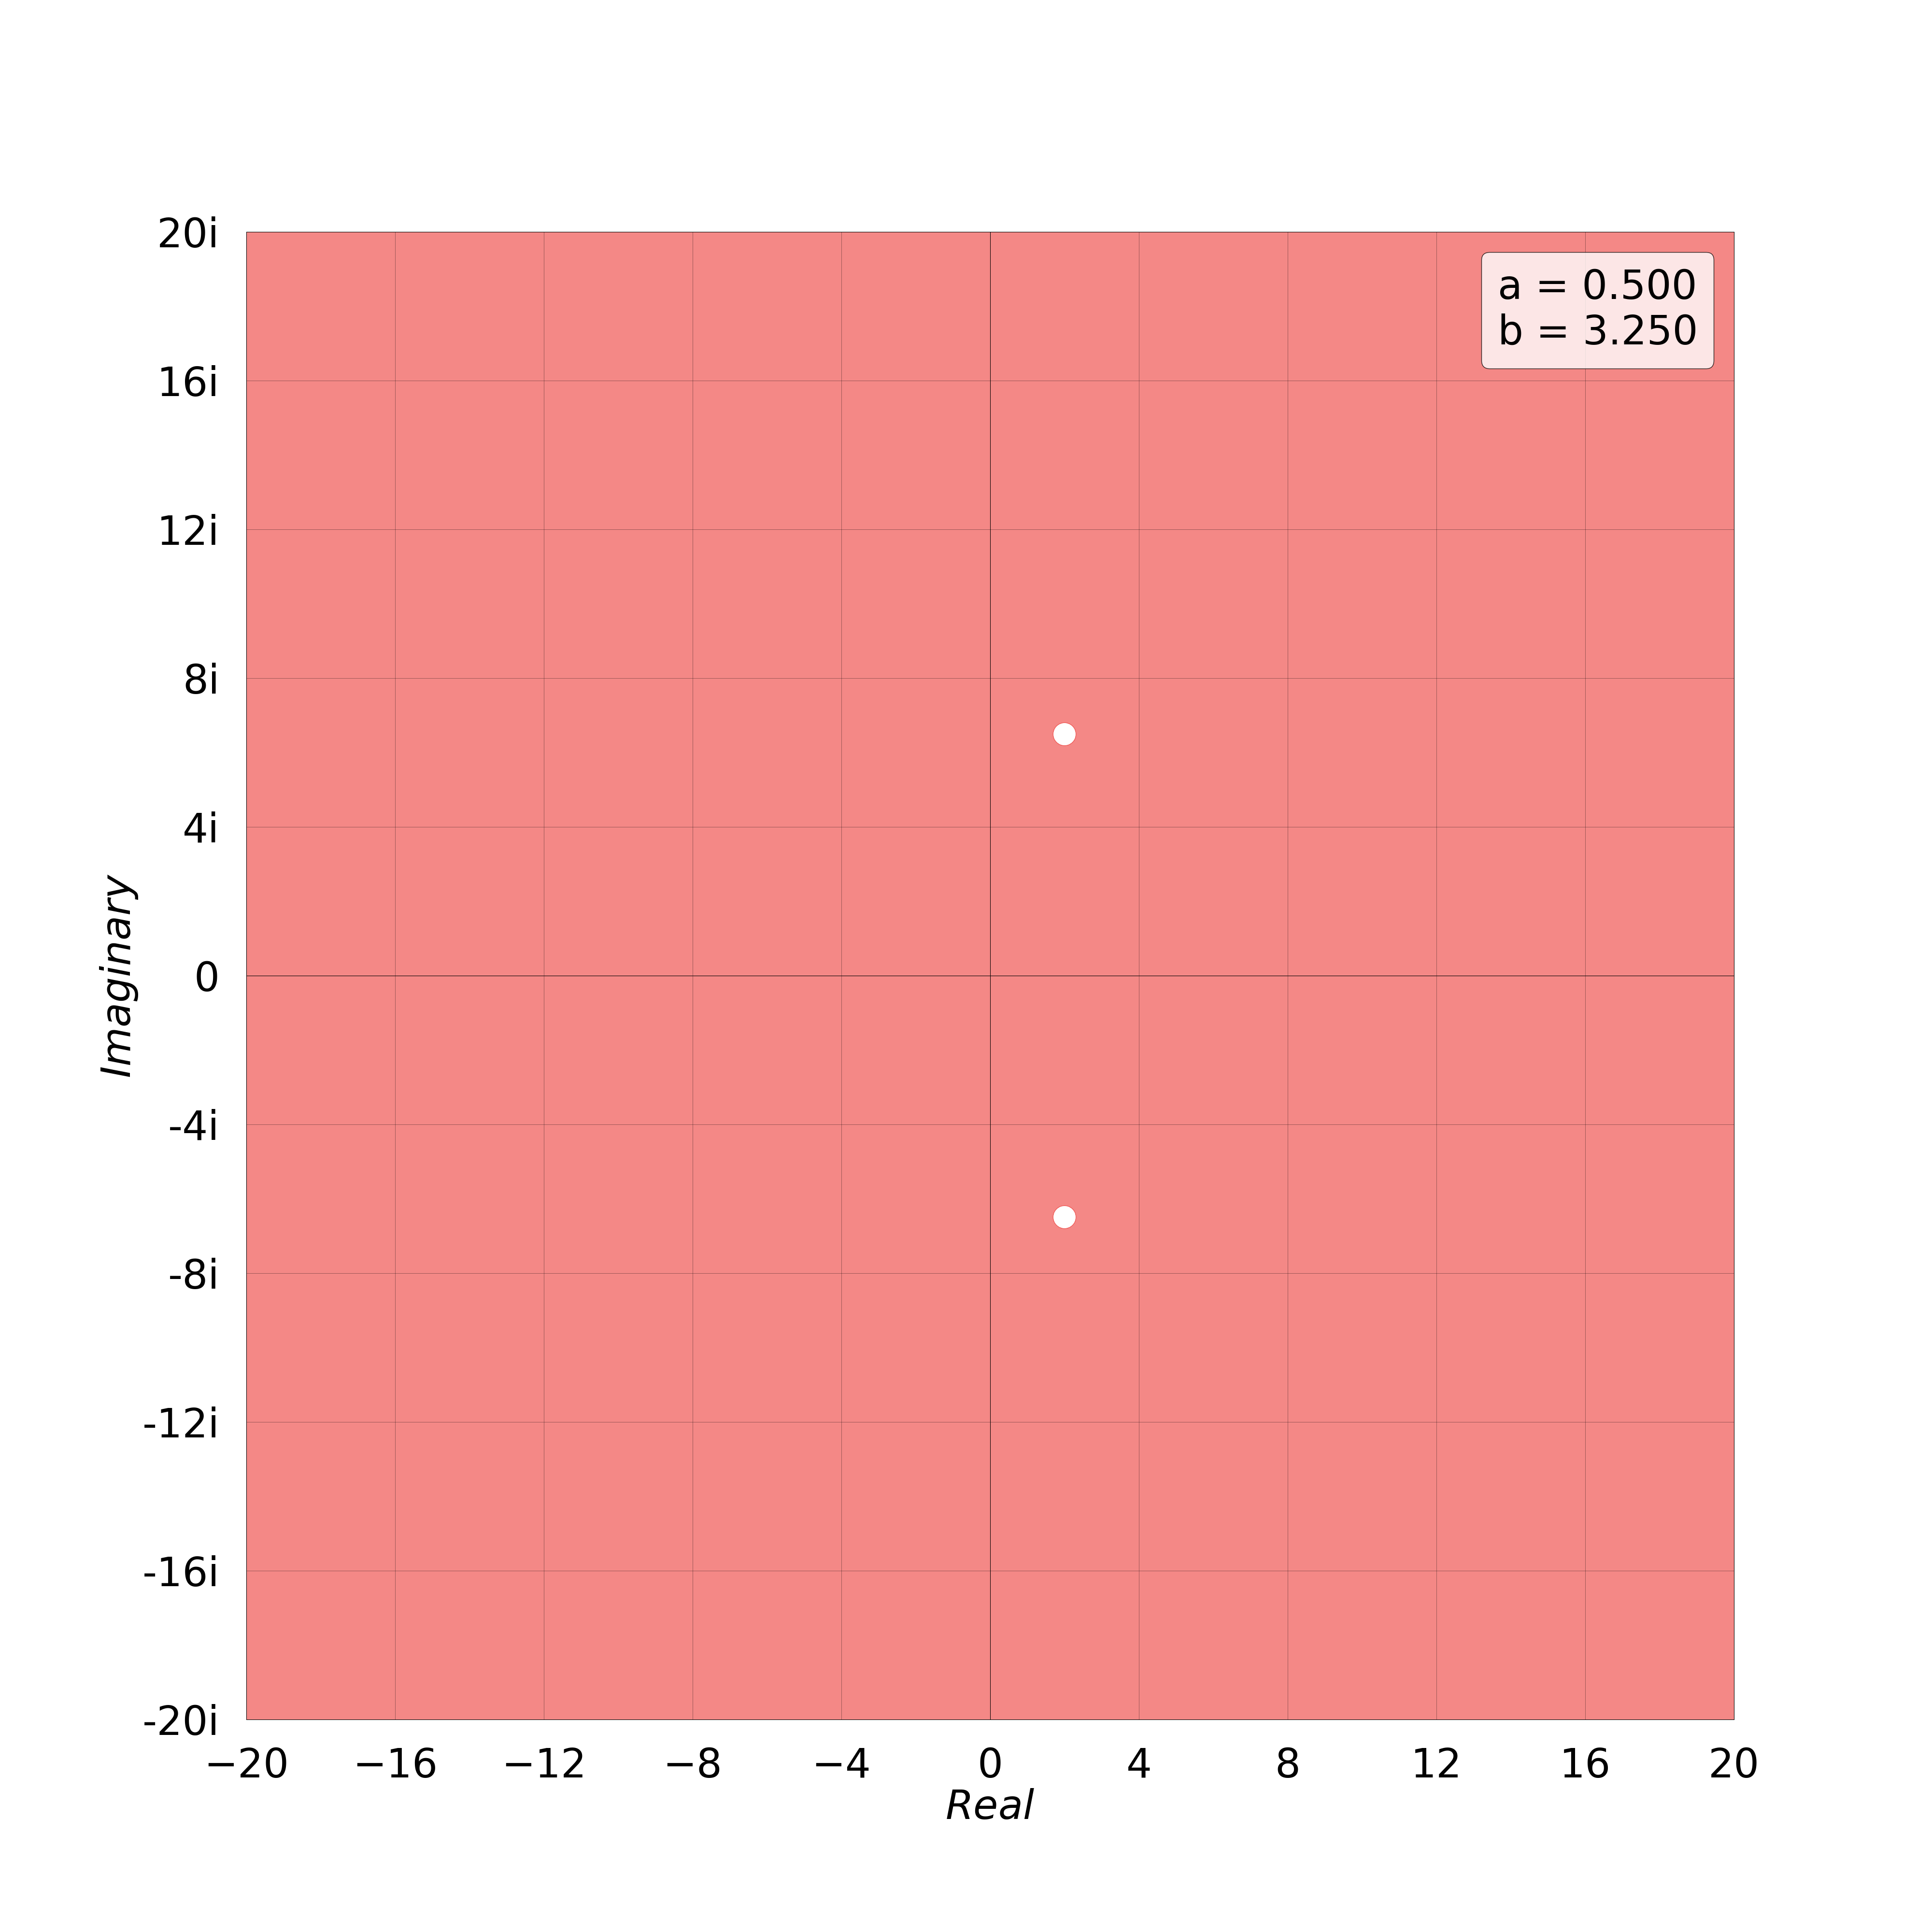
\includegraphics[width=0.32\textwidth]{Stability Regions/Videos/Varied a/Runge-Kutta 4/b=0.5/frames/0650.png}
	\end{center}
\end{multicols}
